\chapter{Development methodology and tools}
\label{chap:methodology}

This chapter aims to introduce the contribution policy and the necessary tools to contribute to the Chromium project.


\section{Development methodology}
Chromium is an open source software project with a specific contribution policy. This is detailed in its official documentation in several sections \cite{contributing,lifeofchromedev,contributingguide}.

The first important detail of the project is that it includes other projects such as v8 \cite{v8} that have their own workflow and, therefore, to contribute to these sections we must review the corresponding documentation. In this case we will focus on the general lines of the Chromium workflow.

The pipeline (figure \ref{fig:contributing_pipeline}) that allows a developer to contribute code to the project goes through: developing the code, creating a change and build it, testing the code, uploading the change for a review and finally committing the patch. If all stages are successfully passed, a satisfactory contribution will have been made.

\begin{figure}
    \centering
    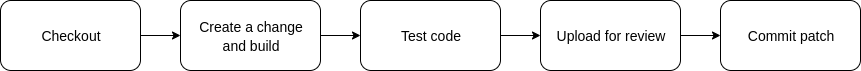
\includegraphics[width=\textwidth]{img/contributing_pipeline.png}
    \caption{Chromium's contributing pipeline.}
    \label{fig:contributing_pipeline}
\end{figure}

\subsection{Initial considerations}

Before delving into details of the contribution pipeline we must pay attention to certain details.

To contribute to the project it is necessary to accept the Contributor License Agreement, which can be individual or corporate depending on the type of contributor. If it is the first contribution, the patch must include a modification of the \texttt{AUTHORS} file so that it includes the name and contact information of the individual or organization that contributes.

It is also important to keep in mind that there is a discussion group as well as various methods to contact developers and code reviewers. It is highly recommended to contact them before getting to work to introduce a new feature or fix a bug.

\subsection{Code checkout}

Chromium is a very large project \footnote{Only the executable file weighs approximately 1.3GB in Linux Debug.}, So we need a slightly powerful machine to work with. To get an idea of the type of machine needed, the documentation indicates that we need a 64-bit machine, even if we are going to build a 32-bit executable, since linking requires more than 4GB of RAM. It is also recommended that the machine has many cores, lots of RAM and a second hard drive for the source code and the building.

If we have that machine, we can proceed to download the source code. The process varies between platforms, but can be summarized in two main points:
\begin{itemize}
    \item Install Depot Tools, a collection of dev utilities.
    \item Run \texttt{fetch chromium} to get all the code and generate the build files.
\end{itemize}

Keep in mind that in order to build in Android it is needed a Linux environment and for iOS it is needed a Mac environment.

\subsubsection{Depot Tools}

Depot Tools is a set of scripts/utilities that:
\begin{itemize}
    \item Manage all checkouts in the Chromium source tree.
    \item Generate the build files for your platform.
    \item Upload your changes to Gerrit \footnote{Used app for the code review process.} for review.
\end{itemize}

\noindent The main utilities for the project are gclient and git-cl.
\begin{description}
\item[gclient] Syncs the source tree and creates build files for your platform.
\item[git-cl] Manages the integration with code review and tryjobs.
\end{description}

\subsection{Modifying and Commiting}

If we have chosen a change to work on, and have discussed it with a senior, we can proceed to follow the Commit Checklist of the project \cite{checklist}.

At the time of writing this document, the checklist steps are:
\begin{enumerate}
    \item \textbf{Create a new branch.} Before starting any development work, it's necessary to create a new branch.
    \item \textbf{Make your changes.} It is important to follow the project code style guide \cite{style_guide}. If the change is going to have a large impact on Chromium it requires a design doc. This design doc has is own review process.
    \item \textbf{Make sure the code builds correctly.} After coding changes, it is necessary to check that common targets build correctly. Note that it's easy to inadvertently break one of the other builds you're not currently working on without realizing it.
    \item \textbf{Test your changes.} For obvious reasons, the code has to be tested. Make sure you cover all code paths you changed.
    \item \textbf{Write unit or browser tests for any new code.} It is recommended to automate every manual test did in the previous stage.
    \item \textbf{Ensure the code is formatted nicely.} Official documentation specifies the \texttt{git cl format {-}{-}js} command \footnote{\texttt{{-}{-}js} option stands for JavaScript supporting.} in order to run the clang auto formatting tools.
    \item \textbf{Check over your changes.} As in the previous stage, the documentation indicates the \texttt{git upstream-diff} in order to check the changes from the most recent checkpoint on the remote repository.
    \item \textbf{Stage relevant files for commit.} Since the project uses git, the relevant files have to be staged for commit using the \texttt{git add} command.
    \item \textbf{Commit your changes.} Use the \texttt{git commit} command. Note that documentation provides some tips for writing proper commit messages.
    \item \textbf{Squash your commits.} When there are a lot of commits made, it is useful to squash the commits in a single commit in order to avoid commit-by-commit merge conflicts.
    \item \textbf{Rebase your local repository.} After commiting, local branches have to be updated with remote changes that have landed since the beginning of the development work. It is also necessary to delete any branch that match the remote repository. This is done by the \texttt{git rebase-update} command. The process can lead into rebase merge conflicts, which should be manually fixed. Since rebasing has the potential to break builds, it is recommended to try re-building after the process.
    \item \textbf{Upload the CL to Gerrit.} This can be done with the \texttt{git cl upload} command.
    \item \textbf{Check the CL again in Gerrit.} The \texttt{git cl web} command takes you to the Gerrit URL associated with the current branch. Here you can check and verify that the uploaded files are correct.
    \item \textbf{Make sure all auto-regression tests pass.} Click \texttt{CQ dry run} and fix any errors. Otherwise the CL won't pass the commit queue (CQ) checks. It is recommended to wait until the CQ Dry run pass before notifying the reviewers since the results may require major changes.
    \item \textbf{Add reviewers to review your code.} There are two ways to do this: you can click \texttt{Find Owners} or run the \texttt{git cl owners} command. Each file with changes in the CL has to be approved by an owner unless you are one of them for some files.
    \item \textbf{Implement feedback from your reviewers.} Reply to all comments from the reviewers on Gerrit and mark all resolved issues as resolved clicking \texttt{Done} or \texttt{Ack}. Click \texttt{Reply} when your CL is ready in order to notify your reviewers that your CL is ready for review again.
    \item \textbf{Land your CL.} Once you have obtained a Code-Review+1 on Gerrit, from at least one owner for each file \footnote{It may be helpful to wait for all your reviewers.}, you are able to land your changes. Click \texttt{Submit to CQ} to try your change in the commit queue (CQ), which will land it if successful.
    \item \textbf{Cleanup.} Run \texttt{git rebase-update} or \texttt{git cl archive} command in order to clean up your local branches. Mark the associated crbug as \texttt{fixed} if proceeds.
\end{enumerate}

If the process landed this point, an official contribution has been made.


\section{Tools}

\subsection{Version Control System}
Chromium uses Git as its VCS. From \cite{git}: 

\textit{``Git is a free and open source distributed version control system designed to handle everything from small to very large projects with speed and efficiency.
Git is easy to learn and has a tiny footprint with lightning fast performance. It outclasses SCM tools like Subversion, CVS, Perforce, and ClearCase with features like cheap local branching, convenient staging areas, and multiple workflows."}

\subsection{Code Review}

Chromium uses Gerrit, a web-based code review tool built on Git. From \cite{gerrit}:

\textit{``Gerrit provides a framework you and your teams can use to review code before it becomes part of the code base. Gerrit works equally well in open source projects that limit the number of users who can approve changes (typical in open source software development) and in projects in which all contributors are trusted."}


\subsection{Recommended IDEs}

The Chromium documentation offers setup guides for a set of recommended IDEs.
\begin{itemize}
    \item Android Studio
    \item Atom
    \item CLion
    \item Eclipse for Android
    \item Eclipse for Linux
    \item EMACS Notes
    \item Qt Creator
    \item Visual Studio Code
\end{itemize}

\subsection{Compiler}

The compiler used in the project is Clang \cite{clang}, a compiler front-end for C family languages. It uses LLVM as back-end and tries to offer an alternative to gcc \cite{gcc}.

\subsection{Communication}

The communication between developers of the project relies on a mailing list and on a Freenode \cite{freenode} channel (\texttt{\#chromium}). Freenode is an IRC \footnote{Real time text-based communication protocol.} network oriented to open source projects in different languages.


\section{Proposed alternatives}

Regarding the development methodology, we can't offer a different solution since we don't know any standard methodology suited for this kind of development. We can agree that the actual methodology is a refined pipeline that evolved from the experience and it is designed to deal with known mistakes.

In the tools point of view, in order to avoid a infrastructural version of the Vendor Lock-In antipattern \cite{lockin}, we propose a set of alternatives:
\begin{itemize}
    \item For the Control Version System we propose Fossil \cite{fossil}, an alternative that shares a lot of features with Git. Its documentation also claims some advantages over Git \cite{fossilvsgit} such as being more efficient and more secure (Fossil uses SHA3 and Git uses SHA2).
    \item For the Code Review task, we propose Phabricator \cite{phabricator}. Some users agree that it works better and is easier to use than Gerrit. On the counterpart, Phabricator is more suited for small and mid size teams while Gerrit is more recommended for big projects as Chromium is.
    \item Since the project just recommends a set of IDEs, we can choose a different tool for developing such as AWS Cloud9 \cite{awscloud9}, a cloud-based IDE that allows you to code, debug and run your code with just a browser.
    \item An alternative for the Clang compiler could be gcc, a wide used and stable compiler for C family languages. Nonetheless, this is just an alternative. Clang seems to fulfill the project requirements and shows some advantages over gcc \cite{clangvsgcc}.
    \item As the team chat software, we propose Slack \cite{slack}. Slack provides integration mechanisms for common services like Trello, GitHub, Dropbox or Mailchimp. The main negative point of Slack is the fact that it is not open source.
\end{itemize}